% Chapter 2: Background and Theoretical Foundations
% Comprehensive IEEE-style textbook chapter on RL for Synthetic Dataset Optimization


This chapter provides the foundational knowledge necessary for understanding the intersection of reinforcement learning, object detection, and synthetic data optimization. We begin with an overview of modern object detection architectures, with particular emphasis on the YOLO family of detectors that have become ubiquitous in real-time applications. We then develop the mathematical framework for reinforcement learning, covering both policy gradient methods and actor-critic architectures essential for continuous optimization problems. The chapter continues with Bayesian optimization as an alternative paradigm, followed by a rigorous treatment of domain randomization theory that underpins sim-to-real transfer. We conclude with multi-fidelity optimization techniques that enable efficient exploration of expensive objective functions.

\section{Object Detection Fundamentals}
\label{sec:object_detection}

Object detection represents one of the fundamental challenges in computer vision, requiring algorithms to simultaneously localize and classify multiple objects within an image. Unlike image classification, which assigns a single label to an entire image, object detection must output a variable number of bounding boxes along with their associated class labels and confidence scores. This task has witnessed remarkable progress over the past decade, driven primarily by advances in deep convolutional neural networks and the availability of large-scale annotated datasets.

\subsection{Two-Stage Versus One-Stage Detectors}
\label{subsec:two_vs_one_stage}

The landscape of modern object detection architectures can be broadly categorized into two paradigms: two-stage detectors and one-stage detectors. Understanding the fundamental differences between these approaches provides essential context for appreciating the design choices made in the YOLO family of detectors.

Two-stage detectors, exemplified by the Region-based Convolutional Neural Network (R-CNN) family, decompose the detection problem into two sequential phases. The first stage generates a sparse set of region proposals that are likely to contain objects of interest. These proposals are generated either through selective search algorithms or, in more modern architectures such as Faster R-CNN, through a Region Proposal Network (RPN) that shares convolutional features with the detection network. The second stage then classifies each proposal and refines the bounding box coordinates through regression. This decomposition allows for high-quality detections by focusing computational resources on promising regions, but introduces latency due to the sequential processing pipeline.

\begin{definition}[Two-Stage Object Detector]
\label{def:two_stage}
A two-stage object detector is a function $\mathcal{D}: \mathcal{I} \rightarrow \mathcal{B}$ that maps an input image $I \in \mathcal{I}$ to a set of detections $\mathcal{B} = \{(b_i, c_i, s_i)\}_{i=1}^{N}$, where $b_i \in \mathbb{R}^4$ represents bounding box coordinates, $c_i \in \{1, \ldots, K\}$ denotes the class label, and $s_i \in [0,1]$ is the confidence score. The detection proceeds through an intermediate representation $\mathcal{R} = \{r_j\}_{j=1}^{M}$ of region proposals, such that $\mathcal{D} = \mathcal{D}_2 \circ \mathcal{D}_1$ where $\mathcal{D}_1: \mathcal{I} \rightarrow \mathcal{R}$ generates proposals and $\mathcal{D}_2: \mathcal{R} \rightarrow \mathcal{B}$ performs classification and refinement.
\end{definition}

One-stage detectors, in contrast, directly predict bounding boxes and class probabilities from the input image in a single forward pass through the network. This architectural simplification eliminates the proposal generation bottleneck and enables real-time inference speeds. The YOLO (You Only Look Once) detector, introduced by Redmon et al. in 2016, pioneered this approach by framing object detection as a regression problem. The input image is divided into a grid, and each grid cell directly predicts bounding boxes and class probabilities for objects whose centers fall within that cell. Single Shot MultiBox Detector (SSD) extended this concept by making predictions at multiple scales using feature maps from different layers of the network.

\begin{definition}[One-Stage Object Detector]
\label{def:one_stage}
A one-stage object detector is a function $\mathcal{D}: \mathcal{I} \rightarrow \mathcal{B}$ that directly maps an input image to detections without intermediate proposal generation. Given a backbone network $\phi: \mathcal{I} \rightarrow \mathcal{F}$ that extracts feature maps and a detection head $\psi: \mathcal{F} \rightarrow \mathcal{B}$, the detector computes $\mathcal{D}(I) = \psi(\phi(I))$ in a single unified network forward pass.
\end{definition}

The trade-off between these paradigms centers on the accuracy-speed continuum. Two-stage detectors typically achieve higher accuracy on challenging benchmarks due to their ability to focus on high-quality proposals, while one-stage detectors offer superior inference speed suitable for real-time applications. Recent advances have narrowed this gap considerably, with modern one-stage detectors achieving competitive accuracy while maintaining their speed advantages.

\begin{figure}[htbp]
\centering
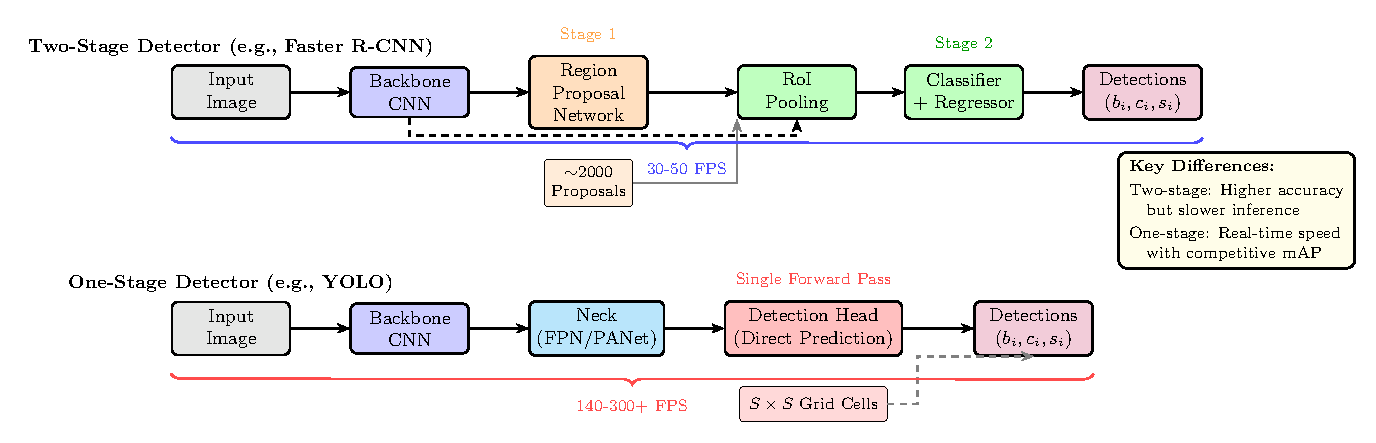
\includegraphics[width=0.95\textwidth]{figures/ch02_fig1_detector_comparison.pdf}
\caption{Architectural comparison between two-stage and one-stage object detectors. Two-stage detectors (top) process images through a Region Proposal Network to generate candidate regions before classification and refinement. One-stage detectors (bottom) directly predict bounding boxes and class probabilities in a single forward pass through the network, enabling significantly higher frame rates at the cost of some accuracy on challenging cases.}
\label{fig:detector_comparison}
\end{figure}

\subsection{Evolution of the YOLO Family}
\label{subsec:yolo_evolution}

The YOLO family of object detectors has undergone substantial evolution since its introduction, with each version incorporating architectural innovations, training improvements, and expanded capabilities. This progression reflects broader trends in deep learning research while maintaining the core philosophy of unified, real-time detection.

YOLOv1, introduced in 2016, established the foundational architecture by dividing images into an $S \times S$ grid, with each cell predicting $B$ bounding boxes and $C$ class probabilities. The network consisted of 24 convolutional layers followed by 2 fully connected layers, inspired by the GoogLeNet architecture. While revolutionary in its approach to real-time detection, YOLOv1 struggled with small objects and objects in close proximity due to the constraint that each grid cell could only predict a limited number of boxes.

YOLOv2, also known as YOLO9000, addressed several limitations of its predecessor through the introduction of batch normalization, anchor boxes derived from clustering on the training data, and multi-scale training. The Darknet-19 backbone replaced the original architecture, providing improved feature extraction while maintaining computational efficiency. The anchor box mechanism allowed the network to leverage prior knowledge about object aspect ratios, significantly improving localization accuracy.

YOLOv3 introduced multi-scale predictions by detecting objects at three different scales using feature pyramid concepts. The backbone evolved to Darknet-53, incorporating residual connections that enabled training of deeper networks. Binary cross-entropy loss replaced softmax for class predictions, enabling multi-label classification where objects could belong to multiple categories simultaneously. These changes substantially improved detection of small objects, which had been a persistent weakness.

YOLOv4 represented a comprehensive study of modern training techniques, incorporating numerous bag-of-freebies and bag-of-specials improvements. The architecture introduced CSPDarknet53 as the backbone, incorporating Cross Stage Partial connections that improved gradient flow while reducing computational cost. Path Aggregation Network (PANet) enhanced feature fusion across scales, while various data augmentation techniques including mosaic augmentation improved generalization. The Mish activation function and other refinements contributed to state-of-the-art accuracy while maintaining real-time performance.

YOLOv5, developed by Ultralytics, transitioned the implementation to PyTorch and introduced a family of models at different scales (nano, small, medium, large, extra-large) to accommodate varying computational budgets. The architecture employed a Focus layer for efficient downsampling and continued refinements to the backbone and neck architectures. Extensive hyperparameter optimization and training recipes contributed to strong out-of-the-box performance across diverse datasets.

YOLOv6 through YOLOv8 continued architectural innovations with efficient reparameterized backbones, decoupled detection heads, and anchor-free designs. YOLOv8 in particular unified detection, segmentation, and pose estimation within a single framework, demonstrating the versatility of the YOLO architecture for multiple vision tasks. The transition to anchor-free detection eliminated the need for hand-designed priors while maintaining detection quality.

YOLOv9 introduced Programmable Gradient Information (PGI) and Generalized Efficient Layer Aggregation Network (GELAN) to address information bottleneck problems in deep networks. These innovations improved gradient flow during training while maintaining inference efficiency, achieving state-of-the-art accuracy on the COCO benchmark.

YOLOv10 and YOLOv11 represent the current frontier, incorporating consistent dual assignments for NMS-free training and attention mechanisms for improved feature aggregation. These versions achieve unprecedented accuracy-latency trade-offs, with YOLOv11 demonstrating particular strength in small object detection and challenging visual conditions.

\begin{table}[htbp]
\centering
\caption{Evolution of YOLO Architectures: Key Characteristics and Performance Metrics}
\label{tab:yolo_comparison}
\begin{tabular}{lccccc}
\toprule
\textbf{Version} & \textbf{Year} & \textbf{Backbone} & \textbf{mAP$_{50}$} & \textbf{FPS} & \textbf{Key Innovation} \\
\midrule
YOLOv1 & 2016 & GoogLeNet-inspired & 63.4 & 45 & Unified detection \\
YOLOv2 & 2017 & Darknet-19 & 78.6 & 67 & Anchor boxes \\
YOLOv3 & 2018 & Darknet-53 & 57.9$^\dagger$ & 30 & Multi-scale prediction \\
YOLOv4 & 2020 & CSPDarknet53 & 65.7$^\dagger$ & 62 & BoF/BoS techniques \\
YOLOv5 & 2020 & CSPDarknet & 68.9$^\dagger$ & 140 & PyTorch ecosystem \\
YOLOv6 & 2022 & EfficientRep & 72.3$^\dagger$ & 175 & Reparameterization \\
YOLOv7 & 2022 & E-ELAN & 73.4$^\dagger$ & 161 & Extended ELAN \\
YOLOv8 & 2023 & CSPDarknet (mod) & 74.0$^\dagger$ & 280 & Anchor-free design \\
YOLOv9 & 2024 & GELAN & 75.5$^\dagger$ & 245 & PGI gradient flow \\
YOLOv10 & 2024 & CSPDarknet-ELAN & 76.1$^\dagger$ & 300 & NMS-free training \\
YOLOv11 & 2024 & C3k2-SPPF & 76.8$^\dagger$ & 320 & Attention mechanisms \\
\bottomrule
\multicolumn{6}{l}{\footnotesize $^\dagger$ mAP measured on COCO val2017 at 640$\times$640 resolution}
\end{tabular}
\end{table}

\subsection{Evaluation Metrics for Object Detection}
\label{subsec:eval_metrics}

Rigorous evaluation of object detection systems requires metrics that capture both localization accuracy and classification performance. The standard metrics employed in the field have evolved to address the unique challenges of evaluating detections across multiple scales and confidence thresholds.

\begin{definition}[Intersection over Union]
\label{def:iou}
The Intersection over Union (IoU), also known as the Jaccard index, measures the overlap between a predicted bounding box $b_p$ and a ground truth bounding box $b_g$:
\begin{equation}
\text{IoU}(b_p, b_g) = \frac{|b_p \cap b_g|}{|b_p \cup b_g|} = \frac{\text{Area of Intersection}}{\text{Area of Union}}
\end{equation}
where $|{\cdot}|$ denotes the area of a region. IoU ranges from 0 (no overlap) to 1 (perfect overlap).
\end{definition}

A detection is considered a true positive if its IoU with a ground truth box exceeds a predefined threshold (commonly 0.5 or 0.75) and the predicted class matches the ground truth class. Multiple detections of the same ground truth object are penalized, with only the highest-confidence detection counted as a true positive and subsequent detections treated as false positives.

\begin{definition}[Precision and Recall]
\label{def:precision_recall}
For a set of detections at a given confidence threshold, precision and recall are defined as:
\begin{equation}
\text{Precision} = \frac{TP}{TP + FP}, \quad \text{Recall} = \frac{TP}{TP + FN}
\end{equation}
where $TP$ denotes true positives (correct detections), $FP$ denotes false positives (incorrect detections or duplicates), and $FN$ denotes false negatives (missed objects).
\end{definition}

The precision-recall curve captures the trade-off between these metrics as the confidence threshold varies. As the threshold decreases, recall typically increases (more objects are detected) while precision may decrease (more false positives are included).

\begin{definition}[Average Precision]
\label{def:ap}
Average Precision (AP) summarizes the precision-recall curve as the area under the curve:
\begin{equation}
\text{AP} = \int_0^1 p(r) \, dr
\end{equation}
where $p(r)$ is the precision at recall level $r$. In practice, this is computed using an $n$-point interpolation:
\begin{equation}
\text{AP} = \frac{1}{n} \sum_{k=1}^{n} p_{\text{interp}}(r_k), \quad p_{\text{interp}}(r_k) = \max_{r \geq r_k} p(r)
\end{equation}
The COCO benchmark uses 101-point interpolation ($n=101$), while earlier benchmarks like PASCAL VOC used 11-point interpolation.
\end{definition}

\begin{definition}[Mean Average Precision]
\label{def:map}
Mean Average Precision (mAP) averages the AP across all $K$ object classes:
\begin{equation}
\text{mAP} = \frac{1}{K} \sum_{k=1}^{K} \text{AP}_k
\end{equation}
The COCO benchmark reports mAP averaged over multiple IoU thresholds from 0.5 to 0.95 in steps of 0.05, denoted mAP$_{50:95}$ or simply mAP. Additional metrics include mAP$_{50}$ (IoU threshold of 0.5) and mAP$_{75}$ (IoU threshold of 0.75), as well as scale-specific metrics mAP$_S$, mAP$_M$, and mAP$_L$ for small, medium, and large objects respectively.
\end{definition}

These metrics provide complementary views of detector performance. High mAP$_{50}$ indicates good object localization at a lenient threshold, while high mAP$_{75}$ requires precise bounding box predictions. The scale-specific metrics reveal performance characteristics across object sizes, which is particularly relevant for applications involving objects at varying distances or scales.

\section{Reinforcement Learning Preliminaries}
\label{sec:rl_preliminaries}

Reinforcement learning provides a principled framework for sequential decision-making under uncertainty, where an agent learns to maximize cumulative reward through interaction with an environment. This section develops the mathematical foundations necessary for applying RL to the optimization of synthetic data generation parameters.

\subsection{Markov Decision Processes}
\label{subsec:mdp}

The Markov Decision Process (MDP) provides the formal framework underlying most reinforcement learning algorithms. An MDP captures the essential elements of sequential decision-making: states, actions, transition dynamics, and rewards.

\begin{definition}[Markov Decision Process]
\label{def:mdp}
A Markov Decision Process is a tuple $\mathcal{M} = (\mathcal{S}, \mathcal{A}, P, R, \gamma)$ where:
\begin{itemize}
\item $\mathcal{S}$ is a set of states (the state space)
\item $\mathcal{A}$ is a set of actions (the action space)
\item $P: \mathcal{S} \times \mathcal{A} \times \mathcal{S} \rightarrow [0,1]$ is the transition probability function, where $P(s'|s,a)$ gives the probability of transitioning to state $s'$ when taking action $a$ in state $s$
\item $R: \mathcal{S} \times \mathcal{A} \rightarrow \mathbb{R}$ is the reward function, where $R(s,a)$ gives the expected immediate reward for taking action $a$ in state $s$
\item $\gamma \in [0,1)$ is the discount factor that determines the relative importance of immediate versus future rewards
\end{itemize}
The Markov property asserts that the future is conditionally independent of the past given the present: $P(s_{t+1}|s_t, a_t, s_{t-1}, a_{t-1}, \ldots) = P(s_{t+1}|s_t, a_t)$.
\end{definition}

The agent's behavior is governed by a policy, which specifies the action selection mechanism in each state.

\begin{definition}[Policy]
\label{def:policy}
A policy $\pi$ maps states to actions or action distributions. A deterministic policy $\pi: \mathcal{S} \rightarrow \mathcal{A}$ specifies a single action for each state. A stochastic policy $\pi: \mathcal{S} \times \mathcal{A} \rightarrow [0,1]$ specifies a probability distribution over actions, where $\pi(a|s)$ denotes the probability of selecting action $a$ in state $s$, satisfying $\sum_{a \in \mathcal{A}} \pi(a|s) = 1$ for all $s$.
\end{definition}

The objective in reinforcement learning is to find a policy that maximizes the expected cumulative discounted reward, known as the return.

\begin{definition}[Return and Value Functions]
\label{def:value_functions}
The return $G_t$ from time $t$ is the discounted sum of future rewards:
\begin{equation}
G_t = \sum_{k=0}^{\infty} \gamma^k R_{t+k+1} = R_{t+1} + \gamma R_{t+2} + \gamma^2 R_{t+3} + \cdots
\end{equation}
The state-value function $V^\pi(s)$ gives the expected return when starting in state $s$ and following policy $\pi$:
\begin{equation}
V^\pi(s) = \mathbb{E}_\pi[G_t | S_t = s] = \mathbb{E}_\pi\left[\sum_{k=0}^{\infty} \gamma^k R_{t+k+1} \Big| S_t = s\right]
\end{equation}
The action-value function $Q^\pi(s,a)$ gives the expected return when starting in state $s$, taking action $a$, and thereafter following policy $\pi$:
\begin{equation}
Q^\pi(s,a) = \mathbb{E}_\pi[G_t | S_t = s, A_t = a] = \mathbb{E}_\pi\left[\sum_{k=0}^{\infty} \gamma^k R_{t+k+1} \Big| S_t = s, A_t = a\right]
\end{equation}
\end{definition}

The value functions satisfy recursive relationships known as Bellman equations, which form the basis for many RL algorithms.

\begin{theorem}[Bellman Equations]
\label{thm:bellman}
For any policy $\pi$, the state-value function satisfies:
\begin{equation}
V^\pi(s) = \sum_{a \in \mathcal{A}} \pi(a|s) \left[ R(s,a) + \gamma \sum_{s' \in \mathcal{S}} P(s'|s,a) V^\pi(s') \right]
\end{equation}
The action-value function satisfies:
\begin{equation}
Q^\pi(s,a) = R(s,a) + \gamma \sum_{s' \in \mathcal{S}} P(s'|s,a) \sum_{a' \in \mathcal{A}} \pi(a'|s') Q^\pi(s',a')
\end{equation}
\end{theorem}

The optimal value functions, denoted $V^*(s)$ and $Q^*(s,a)$, represent the maximum achievable expected return from each state or state-action pair across all possible policies.

\begin{figure}[htbp]
\centering
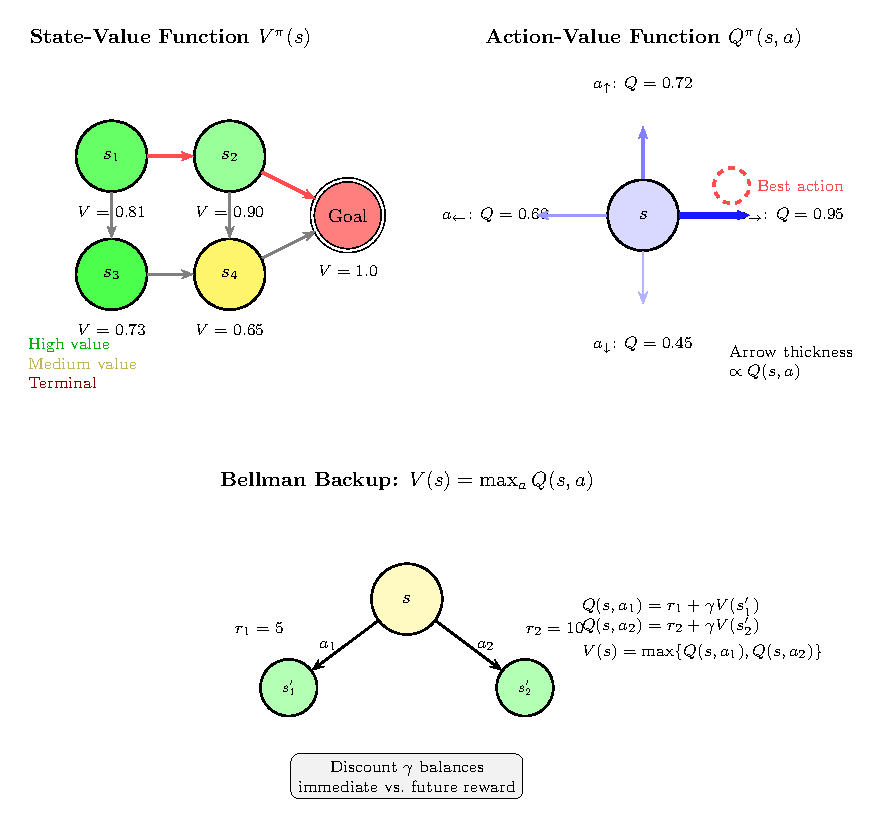
\includegraphics[width=0.9\textwidth]{figures/ch02_fig2_value_function.pdf}
\caption{Visualization of value functions in reinforcement learning. Left: The state-value function $V^\pi(s)$ assigns values to states based on expected future rewards under policy $\pi$. The optimal path (red arrows) follows states with highest values toward the goal. Center: The action-value function $Q^\pi(s,a)$ evaluates each possible action from a state; arrow thickness indicates action quality. Right: The Bellman backup illustrates how value estimates propagate through the state space via the recursive relationship between states and their successors.}
\label{fig:value_functions}
\end{figure}

% TikZ diagram for MDP state-action-reward cycle
\begin{figure}[htbp]
\centering
\begin{tikzpicture}[
    node distance=3cm,
    state/.style={circle, draw, minimum size=1.5cm, thick, fill=blue!10},
    action/.style={rectangle, draw, minimum size=1cm, thick, fill=green!10},
    arrow/.style={->, thick, >=stealth},
    label/.style={font=\small}
]

% Agent node
\node[state] (agent) {Agent};

% Environment node
\node[state, right=5cm of agent] (env) {Environment};

% Action arrow (top)
\draw[arrow, bend left=30] (agent.north east) to node[above, label] {Action $a_t$} (env.north west);

% State arrow (middle)
\draw[arrow, bend left=10] (env.west) to node[below, label, yshift=0.3cm] {State $s_{t+1}$} (agent.east);

% Reward arrow (bottom)
\draw[arrow, bend right=30] (env.south west) to node[below, label] {Reward $r_{t+1}$} (agent.south east);

% Policy annotation
\node[below=0.5cm of agent, align=center, font=\small] {Policy $\pi(a|s)$\\selects actions};

% Dynamics annotation
\node[below=0.5cm of env, align=center, font=\small] {Dynamics $P(s'|s,a)$\\determines transitions};

% Time step annotation
\node[above=1.5cm of agent, xshift=2.5cm, font=\footnotesize] {At each time step $t$:};
\node[above=0.9cm of agent, xshift=2.5cm, font=\footnotesize, align=left] {
1. Agent observes $s_t$\\
2. Agent selects $a_t \sim \pi(\cdot|s_t)$\\
3. Environment returns $r_{t+1}, s_{t+1}$
};

\end{tikzpicture}
\caption{The Markov Decision Process interaction loop. The agent observes the current state from the environment, selects an action according to its policy, and receives a reward along with the next state. This cycle repeats, with the agent's goal being to learn a policy that maximizes cumulative discounted reward.}
\label{fig:mdp_cycle}
\end{figure}

\subsection{Policy Gradient Methods}
\label{subsec:policy_gradient}

Policy gradient methods directly optimize a parameterized policy $\pi_\theta(a|s)$ by estimating gradients of the expected return with respect to the policy parameters $\theta$. These methods are particularly well-suited for continuous action spaces and can naturally handle stochastic policies.

The objective function to maximize is the expected return under the policy:
\begin{equation}
J(\theta) = \mathbb{E}_{\tau \sim \pi_\theta}[R(\tau)] = \mathbb{E}_{\tau \sim \pi_\theta}\left[\sum_{t=0}^{T} \gamma^t r_t\right]
\end{equation}
where $\tau = (s_0, a_0, r_1, s_1, a_1, \ldots)$ denotes a trajectory sampled by following policy $\pi_\theta$.

\begin{theorem}[Policy Gradient Theorem]
\label{thm:policy_gradient}
The gradient of the expected return with respect to policy parameters is:
\begin{equation}
\nabla_\theta J(\theta) = \mathbb{E}_{\tau \sim \pi_\theta}\left[\sum_{t=0}^{T} \nabla_\theta \log \pi_\theta(a_t|s_t) \cdot G_t\right]
\end{equation}
where $G_t = \sum_{k=t}^{T} \gamma^{k-t} r_k$ is the return from time $t$. This can be equivalently expressed as:
\begin{equation}
\nabla_\theta J(\theta) = \mathbb{E}_{s \sim d^\pi, a \sim \pi_\theta}\left[\nabla_\theta \log \pi_\theta(a|s) \cdot Q^{\pi_\theta}(s,a)\right]
\end{equation}
where $d^\pi$ is the stationary state distribution under policy $\pi$.
\end{theorem}

The basic policy gradient estimator, known as REINFORCE, suffers from high variance. Variance reduction techniques include using a baseline function $b(s)$ and the advantage function $A^\pi(s,a) = Q^\pi(s,a) - V^\pi(s)$.

\subsubsection{Trust Region Policy Optimization}

Trust Region Policy Optimization (TRPO) addresses the instability of vanilla policy gradient methods by constraining policy updates to a trust region that ensures monotonic improvement.

\begin{definition}[TRPO Optimization Problem]
\label{def:trpo}
TRPO solves the following constrained optimization problem at each iteration:
\begin{equation}
\begin{aligned}
\max_\theta \quad & \mathbb{E}_{s \sim d^{\pi_{\theta_\text{old}}}, a \sim \pi_{\theta_\text{old}}}\left[\frac{\pi_\theta(a|s)}{\pi_{\theta_\text{old}}(a|s)} A^{\pi_{\theta_\text{old}}}(s,a)\right] \\
\text{s.t.} \quad & \mathbb{E}_{s \sim d^{\pi_{\theta_\text{old}}}}\left[D_\text{KL}(\pi_{\theta_\text{old}}(\cdot|s) \| \pi_\theta(\cdot|s))\right] \leq \delta
\end{aligned}
\end{equation}
where $D_\text{KL}$ denotes the Kullback-Leibler divergence and $\delta$ is the trust region constraint.
\end{definition}

TRPO uses conjugate gradient descent and line search to approximately solve this constrained optimization problem, requiring computation of the Fisher information matrix.

\subsubsection{Proximal Policy Optimization}

Proximal Policy Optimization (PPO) simplifies TRPO by replacing the hard KL constraint with a clipped surrogate objective that achieves similar trust region effects without the computational complexity.

\begin{definition}[PPO Clipped Objective]
\label{def:ppo}
PPO maximizes the clipped surrogate objective:
\begin{equation}
L^\text{CLIP}(\theta) = \mathbb{E}_t\left[\min\left(r_t(\theta) \hat{A}_t, \text{clip}(r_t(\theta), 1-\epsilon, 1+\epsilon) \hat{A}_t\right)\right]
\end{equation}
where $r_t(\theta) = \frac{\pi_\theta(a_t|s_t)}{\pi_{\theta_\text{old}}(a_t|s_t)}$ is the probability ratio, $\hat{A}_t$ is an advantage estimate, and $\epsilon$ (typically 0.2) controls the clipping range.
\end{definition}

The clipping mechanism removes the incentive for moving the policy ratio outside the interval $[1-\epsilon, 1+\epsilon]$, effectively constraining the policy update. When the advantage is positive, the objective encourages increasing the probability of the action, but clips the benefit once $r_t(\theta) > 1+\epsilon$. When the advantage is negative, the objective encourages decreasing the probability, but clips once $r_t(\theta) < 1-\epsilon$.

\begin{algorithm}[htbp]
\caption{Proximal Policy Optimization (PPO)}
\label{alg:ppo}
\begin{algorithmic}[1]
\Require Initial policy parameters $\theta_0$, initial value function parameters $\phi_0$
\Require Clipping parameter $\epsilon$, number of epochs $K$, minibatch size $M$
\For{iteration $= 1, 2, \ldots$}
    \State Collect set of trajectories $\mathcal{D}_k$ by running policy $\pi_{\theta_k}$ in environment
    \State Compute rewards-to-go $\hat{R}_t$ for all timesteps in $\mathcal{D}_k$
    \State Compute advantage estimates $\hat{A}_t$ using GAE or other estimator
    \State Normalize advantages: $\hat{A}_t \leftarrow (\hat{A}_t - \mu_A) / \sigma_A$
    \For{epoch $= 1, \ldots, K$}
        \For{minibatch $\mathcal{B} \subset \mathcal{D}_k$ of size $M$}
            \State Compute policy ratio $r_t(\theta) = \pi_\theta(a_t|s_t) / \pi_{\theta_k}(a_t|s_t)$
            \State Compute clipped objective: $L^\text{CLIP} = \frac{1}{|\mathcal{B}|}\sum_t \min(r_t \hat{A}_t, \text{clip}(r_t, 1{\pm}\epsilon) \hat{A}_t)$
            \State Compute value loss: $L^\text{VF} = \frac{1}{|\mathcal{B}|}\sum_t (V_\phi(s_t) - \hat{R}_t)^2$
            \State Update $\theta$ by gradient ascent on $L^\text{CLIP}$
            \State Update $\phi$ by gradient descent on $L^\text{VF}$
        \EndFor
    \EndFor
\EndFor
\end{algorithmic}
\end{algorithm}

PPO has become the de facto standard for policy gradient methods due to its simplicity, stability, and competitive performance across a wide range of tasks. Its on-policy nature means that data collected under the current policy must be discarded after each update, which can limit sample efficiency in settings where environment interactions are expensive.

\subsection{Actor-Critic Architectures}
\label{subsec:actor_critic}

Actor-critic methods combine policy gradient approaches with value function estimation, using a learned value function (the critic) to reduce variance in policy gradient estimates while maintaining the flexibility of policy-based methods (the actor).

\begin{figure}[htbp]
\centering
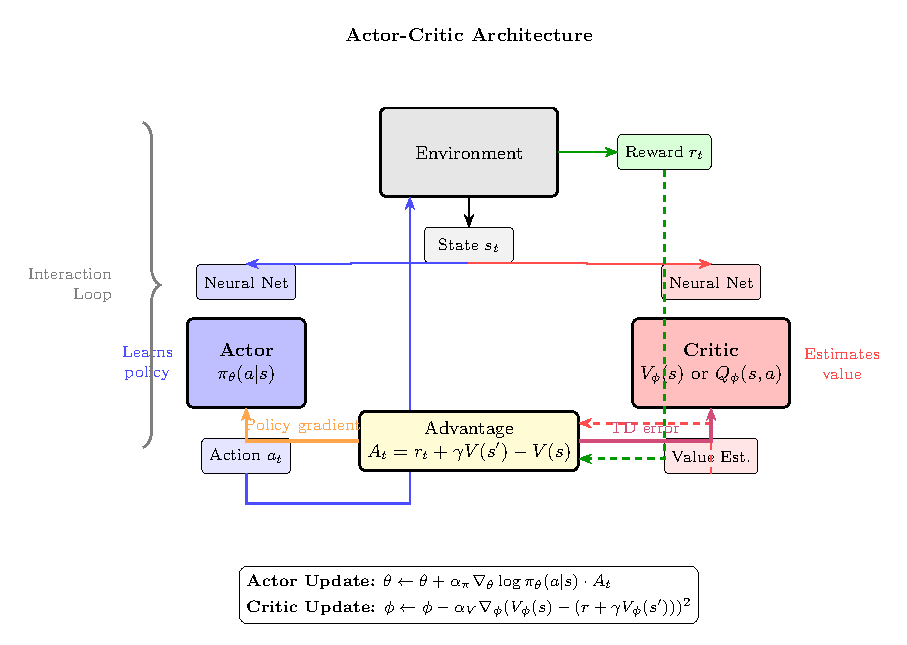
\includegraphics[width=0.85\textwidth]{figures/ch02_fig3_actor_critic.pdf}
\caption{The actor-critic architecture. The actor network learns a policy $\pi_\theta(a|s)$ that maps states to action distributions, while the critic network estimates the value function $V_\phi(s)$ or action-value function $Q_\phi(s,a)$. The temporal difference error computed from the critic's estimates provides a low-variance learning signal for updating the actor's policy parameters. This architecture combines the stability benefits of value-based methods with the flexibility of policy gradient approaches.}
\label{fig:actor_critic}
\end{figure}

\subsubsection{Soft Actor-Critic}

Soft Actor-Critic (SAC) is an off-policy actor-critic algorithm that incorporates entropy regularization to encourage exploration and improve robustness. The maximum entropy framework augments the standard RL objective with an entropy term.

\begin{definition}[Maximum Entropy Objective]
\label{def:max_entropy}
The maximum entropy reinforcement learning objective is:
\begin{equation}
J(\pi) = \sum_{t=0}^{T} \mathbb{E}_{(s_t, a_t) \sim \rho_\pi}\left[r(s_t, a_t) + \alpha \mathcal{H}(\pi(\cdot|s_t))\right]
\end{equation}
where $\mathcal{H}(\pi(\cdot|s)) = -\sum_a \pi(a|s) \log \pi(a|s)$ is the entropy of the policy and $\alpha > 0$ is the temperature parameter controlling the entropy-reward trade-off.
\end{definition}

SAC maintains three function approximators: a policy network $\pi_\theta$, and two Q-function networks $Q_{\phi_1}$, $Q_{\phi_2}$ (using the minimum to address overestimation bias). The soft value functions incorporate the entropy term.

\begin{definition}[Soft Bellman Equation]
\label{def:soft_bellman}
The soft Q-function satisfies the soft Bellman equation:
\begin{equation}
Q(s_t, a_t) = r(s_t, a_t) + \gamma \mathbb{E}_{s_{t+1}}\left[V(s_{t+1})\right]
\end{equation}
where the soft value function is:
\begin{equation}
V(s_t) = \mathbb{E}_{a_t \sim \pi}\left[Q(s_t, a_t) - \alpha \log \pi(a_t|s_t)\right]
\end{equation}
\end{definition}

SAC's off-policy nature allows it to reuse past experience stored in a replay buffer, providing substantial sample efficiency improvements over on-policy methods. The entropy regularization prevents premature convergence and maintains exploration throughout training.

\begin{algorithm}[htbp]
\caption{Soft Actor-Critic (SAC)}
\label{alg:sac}
\begin{algorithmic}[1]
\Require Initial policy parameters $\theta$, Q-function parameters $\phi_1, \phi_2$
\Require Target Q-function parameters $\bar{\phi}_1 \leftarrow \phi_1$, $\bar{\phi}_2 \leftarrow \phi_2$
\Require Empty replay buffer $\mathcal{D}$, learning rates $\lambda_Q$, $\lambda_\pi$, $\lambda_\alpha$
\For{each iteration}
    \For{each environment step}
        \State Sample action $a_t \sim \pi_\theta(\cdot|s_t)$
        \State Execute $a_t$, observe $r_t$, $s_{t+1}$
        \State Store $(s_t, a_t, r_t, s_{t+1})$ in $\mathcal{D}$
    \EndFor
    \For{each gradient step}
        \State Sample minibatch $\mathcal{B} = \{(s, a, r, s')\}$ from $\mathcal{D}$
        \State Compute target: $y = r + \gamma(\min_{i=1,2} Q_{\bar{\phi}_i}(s', \tilde{a}') - \alpha \log \pi_\theta(\tilde{a}'|s'))$ where $\tilde{a}' \sim \pi_\theta(\cdot|s')$
        \State Update Q-functions: $\phi_i \leftarrow \phi_i - \lambda_Q \nabla_{\phi_i} \frac{1}{|\mathcal{B}|}\sum(Q_{\phi_i}(s,a) - y)^2$
        \State Update policy: $\theta \leftarrow \theta + \lambda_\pi \nabla_\theta \frac{1}{|\mathcal{B}|}\sum(\alpha \log \pi_\theta(\tilde{a}|s) - \min_{i} Q_{\phi_i}(s, \tilde{a}))$
        \State Update temperature: $\alpha \leftarrow \alpha - \lambda_\alpha \nabla_\alpha \frac{1}{|\mathcal{B}|}\sum(-\alpha \log \pi_\theta(\tilde{a}|s) - \alpha \bar{\mathcal{H}})$
        \State Update targets: $\bar{\phi}_i \leftarrow \tau \phi_i + (1-\tau)\bar{\phi}_i$
    \EndFor
\EndFor
\end{algorithmic}
\end{algorithm}

\subsubsection{Twin Delayed Deep Deterministic Policy Gradient}

Twin Delayed Deep Deterministic Policy Gradient (TD3) addresses overestimation bias and instability in deterministic policy gradient methods through three key modifications: clipped double Q-learning, delayed policy updates, and target policy smoothing.

\begin{definition}[TD3 Modifications]
\label{def:td3}
TD3 incorporates three modifications to DDPG:
\begin{enumerate}
\item \textbf{Clipped Double Q-learning}: Use the minimum of two Q-networks for computing the target:
\begin{equation}
y = r + \gamma \min_{i=1,2} Q_{\bar{\phi}_i}(s', \pi_{\bar{\theta}}(s'))
\end{equation}
\item \textbf{Delayed Policy Updates}: Update the policy network less frequently than the Q-networks (typically every 2 Q-updates).
\item \textbf{Target Policy Smoothing}: Add noise to target actions to prevent exploitation of Q-function errors:
\begin{equation}
\tilde{a}' = \pi_{\bar{\theta}}(s') + \text{clip}(\epsilon, -c, c), \quad \epsilon \sim \mathcal{N}(0, \sigma^2)
\end{equation}
\end{enumerate}
\end{definition}

TD3 is particularly effective for continuous control tasks where deterministic policies are appropriate. The combination of techniques provides more stable learning than DDPG while maintaining its sample efficiency advantages.

\subsection{Off-Policy Versus On-Policy Learning}
\label{subsec:off_on_policy}

The distinction between off-policy and on-policy learning has significant implications for sample efficiency, stability, and applicability to different problem settings.

On-policy methods, including REINFORCE, A2C, TRPO, and PPO, learn from data collected under the current policy. After each policy update, previously collected data becomes stale and must be discarded because the importance weights required for off-policy correction become highly variable. This constraint limits sample efficiency but provides stable learning dynamics and unbiased gradient estimates.

Off-policy methods, including DQN, DDPG, SAC, and TD3, can learn from data collected under any policy, enabling the use of experience replay buffers that store past transitions. This dramatically improves sample efficiency by allowing each transition to contribute to multiple gradient updates. However, off-policy learning introduces challenges including the deadly triad (function approximation, bootstrapping, and off-policy learning) that can lead to instability.

\begin{table}[htbp]
\centering
\caption{Comparison of On-Policy and Off-Policy Reinforcement Learning}
\label{tab:on_off_policy}
\begin{tabular}{lcc}
\toprule
\textbf{Characteristic} & \textbf{On-Policy} & \textbf{Off-Policy} \\
\midrule
Sample efficiency & Lower & Higher \\
Learning stability & More stable & Can be unstable \\
Experience replay & Not directly usable & Fully utilized \\
Exploration & Via policy stochasticity & Via replay diversity \\
Gradient bias & Unbiased & Requires correction \\
Representative algorithms & PPO, TRPO, A2C & SAC, TD3, DQN \\
\bottomrule
\end{tabular}
\end{table}

For the problem of optimizing synthetic data generation parameters, sample efficiency is paramount because each evaluation requires training a detection model, a computationally expensive operation. This consideration favors off-policy methods such as SAC, though the relatively low-dimensional action space (generator parameters) may also make sample-efficient variants of on-policy methods viable.

\section{Bayesian Optimization}
\label{sec:bayesian_optimization}

Bayesian optimization provides an alternative paradigm for black-box optimization that is particularly well-suited for expensive objective functions. Unlike reinforcement learning, which learns a policy for sequential decision-making, Bayesian optimization directly models the objective function and uses this model to guide the search for optimal parameters.

\subsection{Gaussian Processes as Surrogate Models}
\label{subsec:gaussian_processes}

The core idea of Bayesian optimization is to construct a probabilistic surrogate model of the objective function based on observed evaluations, then use this model to decide where to evaluate next. Gaussian Processes (GPs) are the most common choice for surrogate models due to their flexibility and principled uncertainty quantification.

\begin{definition}[Gaussian Process]
\label{def:gp}
A Gaussian Process is a collection of random variables, any finite number of which have a joint Gaussian distribution. A GP is fully specified by its mean function $m(x)$ and covariance function (kernel) $k(x, x')$:
\begin{equation}
f(x) \sim \mathcal{GP}(m(x), k(x, x'))
\end{equation}
where $m(x) = \mathbb{E}[f(x)]$ and $k(x, x') = \mathbb{E}[(f(x) - m(x))(f(x') - m(x'))]$.
\end{definition}

Given observations $\mathcal{D} = \{(x_i, y_i)\}_{i=1}^{n}$ where $y_i = f(x_i) + \epsilon$ with $\epsilon \sim \mathcal{N}(0, \sigma^2_n)$, the posterior distribution over function values at a new point $x_*$ is Gaussian:
\begin{equation}
f(x_*) | \mathcal{D} \sim \mathcal{N}(\mu(x_*), \sigma^2(x_*))
\end{equation}
with posterior mean and variance:
\begin{align}
\mu(x_*) &= m(x_*) + k(x_*, X)(K + \sigma^2_n I)^{-1}(y - m(X)) \\
\sigma^2(x_*) &= k(x_*, x_*) - k(x_*, X)(K + \sigma^2_n I)^{-1}k(X, x_*)
\end{align}
where $K$ is the kernel matrix with $K_{ij} = k(x_i, x_j)$.

The choice of kernel encodes prior assumptions about the function's properties. The squared exponential (RBF) kernel $k(x, x') = \sigma^2_f \exp\left(-\frac{\|x-x'\|^2}{2\ell^2}\right)$ assumes smooth functions, while the Mat\'{e}rn kernel allows control over differentiability.

\subsection{Acquisition Functions}
\label{subsec:acquisition_functions}

Acquisition functions use the posterior distribution to quantify the utility of evaluating the objective at different points, balancing exploration of uncertain regions with exploitation of promising areas.

\begin{definition}[Expected Improvement]
\label{def:ei}
Expected Improvement (EI) measures the expected amount by which a new evaluation will improve upon the current best observation $f^* = \max_{i} y_i$:
\begin{equation}
\text{EI}(x) = \mathbb{E}[\max(f(x) - f^*, 0)] = (μ(x) - f^*)\Phi(Z) + \sigma(x)\phi(Z)
\end{equation}
where $Z = \frac{\mu(x) - f^*}{\sigma(x)}$, and $\Phi$, $\phi$ are the CDF and PDF of the standard normal distribution.
\end{definition}

\begin{definition}[Upper Confidence Bound]
\label{def:ucb}
Upper Confidence Bound (UCB) selects points that maximize an optimistic estimate of the function value:
\begin{equation}
\text{UCB}(x) = \mu(x) + \beta \sigma(x)
\end{equation}
where $\beta > 0$ controls the exploration-exploitation trade-off. Larger $\beta$ favors exploration of uncertain regions.
\end{definition}

Other acquisition functions include Probability of Improvement (PI), Thompson Sampling, and Knowledge Gradient. The optimal acquisition function depends on problem characteristics including noise level, evaluation budget, and the relative costs of exploration versus exploitation.

% TikZ diagram for Gaussian Process with acquisition function
\begin{figure}[htbp]
\centering
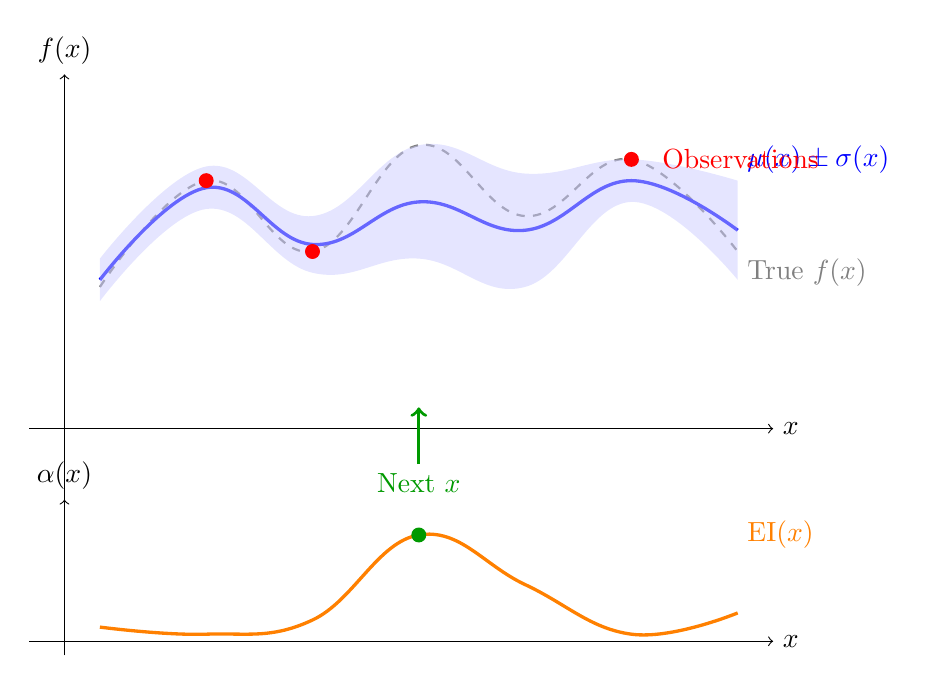
\begin{tikzpicture}[scale=0.9]
    % Draw axes
    \draw[->] (-0.5, 0) -- (10, 0) node[right] {$x$};
    \draw[->] (0, -1) -- (0, 5) node[above] {$f(x)$};

    % True function (hidden, dashed)
    \draw[dashed, gray, thick] plot[smooth, tension=0.7] coordinates {
        (0.5, 2) (2, 3.5) (3.5, 2.5) (5, 4) (6.5, 3) (8, 3.8) (9.5, 2.5)
    };

    % GP mean function
    \draw[blue, very thick] plot[smooth, tension=0.7] coordinates {
        (0.5, 2.1) (2, 3.4) (3.5, 2.6) (5, 3.2) (6.5, 2.8) (8, 3.5) (9.5, 2.8)
    };

    % GP uncertainty (shaded region)
    \fill[blue!20, opacity=0.5] plot[smooth, tension=0.7] coordinates {
        (0.5, 2.4) (2, 3.7) (3.5, 3.0) (5, 4.0) (6.5, 3.6) (8, 3.8) (9.5, 3.5)
    } -- plot[smooth, tension=0.7] coordinates {
        (9.5, 2.1) (8, 3.2) (6.5, 2.0) (5, 2.4) (3.5, 2.2) (2, 3.1) (0.5, 1.8)
    } -- cycle;

    % Observed points
    \fill[red] (2, 3.5) circle (3pt);
    \fill[red] (3.5, 2.5) circle (3pt);
    \fill[red] (8, 3.8) circle (3pt);

    % Next evaluation point (from acquisition function)
    \draw[green!60!black, very thick, ->] (5, -0.5) -- (5, 0.3);
    \node[green!60!black, below] at (5, -0.5) {Next $x$};

    % Acquisition function (bottom subplot)
    \begin{scope}[yshift=-3cm]
        \draw[->] (-0.5, 0) -- (10, 0) node[right] {$x$};
        \draw[->] (0, -0.2) -- (0, 2) node[above] {$\alpha(x)$};

        % EI acquisition function
        \draw[orange, very thick] plot[smooth, tension=0.7] coordinates {
            (0.5, 0.2) (2, 0.1) (3.5, 0.3) (5, 1.5) (6.5, 0.8) (8, 0.1) (9.5, 0.4)
        };

        % Maximum of acquisition function
        \fill[green!60!black] (5, 1.5) circle (3pt);
    \end{scope}

    % Labels
    \node[blue, right] at (9.5, 3.8) {$\mu(x) \pm \sigma(x)$};
    \node[gray, right] at (9.5, 2.2) {True $f(x)$};
    \node[red, right] at (8.3, 3.8) {Observations};
    \node[orange, right] at (9.5, -1.5) {EI$(x)$};

\end{tikzpicture}
\caption{Bayesian optimization with a Gaussian Process surrogate model. The top panel shows the GP posterior mean (blue line) with uncertainty bounds (shaded region) based on three observations (red points). The dashed gray line represents the unknown true function. The bottom panel shows the Expected Improvement acquisition function, which peaks at regions of high uncertainty and predicted improvement. The next evaluation point is selected at the acquisition function maximum.}
\label{fig:gp_acquisition}
\end{figure}

\subsection{The Exploration-Exploitation Trade-off}
\label{subsec:exploration_exploitation}

The exploration-exploitation trade-off is fundamental to both Bayesian optimization and reinforcement learning, though it manifests differently in each setting.

In Bayesian optimization, exploration refers to evaluating points where the surrogate model has high uncertainty, potentially discovering better regions of the search space. Exploitation refers to evaluating points where the model predicts high objective values, refining the estimate of the optimum. Acquisition functions implicitly balance these objectives: EI naturally incorporates both through its dependence on both the mean (exploitation) and variance (exploration), while UCB provides explicit control through the $\beta$ parameter.

\begin{theorem}[Regret Bounds for GP-UCB]
\label{thm:gp_ucb_regret}
For a function $f$ sampled from a GP with bounded RKHS norm, the GP-UCB algorithm with appropriately chosen $\beta_t$ achieves sublinear cumulative regret:
\begin{equation}
R_T = \sum_{t=1}^{T} (f(x^*) - f(x_t)) = \mathcal{O}^*(\sqrt{T \gamma_T})
\end{equation}
where $\gamma_T$ is the maximum information gain and $\mathcal{O}^*$ hides logarithmic factors. For the squared exponential kernel in $d$ dimensions, $\gamma_T = \mathcal{O}((\log T)^{d+1})$.
\end{theorem}

This theoretical guarantee ensures that Bayesian optimization converges to the optimum, with the rate depending on the complexity of the function class through the information gain term.

\subsection{Comparison with Reinforcement Learning Approaches}
\label{subsec:bo_vs_rl}

Bayesian optimization and reinforcement learning offer complementary approaches to the problem of optimizing synthetic data generator parameters. Understanding their relative strengths guides the selection of appropriate methods.

Bayesian optimization excels when the objective function is expensive to evaluate, the parameter space is relatively low-dimensional (typically fewer than 20 dimensions), and the optimization is stateless (each evaluation is independent). The method provides principled uncertainty quantification and achieves strong theoretical guarantees on sample efficiency.

Reinforcement learning is preferred when the optimization involves sequential decision-making with state dependence, the action space is high-dimensional, or the problem structure allows for policy generalization across similar tasks. RL can also leverage partial feedback and intermediate rewards, which may not be available in pure black-box optimization.

For synthetic data optimization, both approaches have merit. The problem can be framed as stateless black-box optimization (favoring BO) if we optimize generator parameters for a single training run, or as sequential decision-making (favoring RL) if we adaptively adjust parameters during the course of dataset generation based on observed detection performance.

\begin{table}[htbp]
\centering
\caption{Comparison of Bayesian Optimization and Reinforcement Learning for Parameter Optimization}
\label{tab:bo_vs_rl}
\begin{tabular}{lcc}
\toprule
\textbf{Characteristic} & \textbf{Bayesian Optimization} & \textbf{Reinforcement Learning} \\
\midrule
Problem structure & Stateless, black-box & Sequential, state-dependent \\
Dimensionality & Low ($\lesssim 20$) & Higher tolerated \\
Sample efficiency & Very high & Moderate to high \\
Uncertainty quantification & Principled (GP posterior) & Implicit (policy entropy) \\
Intermediate feedback & Not utilized & Can be leveraged \\
Theoretical guarantees & Strong (regret bounds) & Weaker (convergence) \\
Parallelization & Batch acquisition & Distributed rollouts \\
\bottomrule
\end{tabular}
\end{table}

Hybrid approaches combining elements of both paradigms have shown promise. BOHB (Bayesian Optimization HyperBand) combines Bayesian optimization with multi-fidelity evaluation, while methods like Neural Architecture Search use RL to search over discrete structures with BO for continuous hyperparameters.

\section{Domain Randomization Theory}
\label{sec:domain_randomization}

Domain randomization has emerged as a powerful technique for training models on synthetic data that transfer effectively to real-world settings. This section develops the theoretical foundations of domain randomization, drawing on recent work that provides formal guarantees for sim-to-real transfer.

\subsection{Formal Framework for Domain Randomization}
\label{subsec:dr_framework}

The theoretical framework for understanding domain randomization models the simulator as a family of environments parameterized by unknown physical and visual parameters. The key insight is that by training on a sufficiently diverse distribution over these parameters, the policy learns to be robust to the specific parameter values encountered in the real world.

\begin{definition}[Domain Randomization Framework]
\label{def:dr_framework}
Consider a family of MDPs $\{\mathcal{M}_\xi\}_{\xi \in \Xi}$ indexed by domain parameters $\xi$ (representing physical properties, visual appearance, etc.). Let $P_\Xi$ be a distribution over domain parameters. Domain randomization trains a policy $\pi$ on the mixture MDP:
\begin{equation}
\mathcal{M}_{DR} = \int_\Xi \mathcal{M}_\xi \, dP_\Xi(\xi)
\end{equation}
The goal is that a policy performing well under $\mathcal{M}_{DR}$ will also perform well on the real-world MDP $\mathcal{M}_{\xi^*}$ for unknown $\xi^* \in \Xi$.
\end{definition}

The ICLR 2022 paper ``Understanding Domain Randomization for Sim-to-real Transfer'' established formal conditions under which domain randomization succeeds. The key result demonstrates that under mild assumptions, domain randomization can achieve zero-shot transfer without any real-world training data.

\begin{theorem}[Domain Randomization Transfer]
\label{thm:dr_transfer}
Let $\pi^*_{DR}$ be an optimal policy for the domain-randomized MDP $\mathcal{M}_{DR}$, and let $\mathcal{M}_{\xi^*}$ be the real-world MDP with $\xi^* \in \Xi$. Under the assumption that the optimal Q-function varies smoothly with domain parameters, the performance gap satisfies:
\begin{equation}
V^*_{\xi^*} - V^{\pi^*_{DR}}_{\xi^*} \leq C \cdot d(\xi^*, \text{supp}(P_\Xi))
\end{equation}
where $V^*_{\xi^*}$ is the optimal value in the real world, $V^{\pi^*_{DR}}_{\xi^*}$ is the value of the domain-randomized policy in the real world, $C$ is a Lipschitz constant, and $d(\cdot, \cdot)$ measures distance to the support of the randomization distribution.
\end{theorem}

This theorem provides a formal justification for domain randomization: if the randomization distribution $P_\Xi$ has support containing or near the real-world parameters $\xi^*$, the transfer gap is bounded.

\subsection{Why Randomization Enables Generalization}
\label{subsec:why_randomization}

The effectiveness of domain randomization can be understood through several complementary perspectives that illuminate why introducing variability in synthetic data improves generalization to real-world conditions.

From a robustness perspective, training on diverse domain parameters forces the policy to rely on features that are consistent across variations rather than domain-specific artifacts. For object detection, this means learning to recognize objects based on their shape and geometric structure rather than spurious correlations with specific textures, lighting conditions, or background patterns.

From a coverage perspective, sufficient randomization ensures that the real-world domain appears as ``just another variation'' within the training distribution. If the randomization spans a sufficiently wide range of visual and physical parameters, the gap between simulation and reality becomes a small perturbation that well-trained models can tolerate.

From a regularization perspective, domain randomization acts as a form of implicit regularization that prevents overfitting to specific characteristics of the simulated environment. This is analogous to data augmentation techniques in supervised learning, but applied at the level of the entire rendering and physics pipeline rather than individual images.

The theoretical framework also highlights the importance of using memory or recurrent policies when dealing with partially observable domains. Memoryless policies cannot distinguish between different domain parameters from single observations, which can lead to suboptimal behavior. History-dependent policies can implicitly infer domain characteristics from sequences of observations and adapt their behavior accordingly.

\subsection{Structured Versus Unstructured Randomization}
\label{subsec:structured_unstructured}

A critical distinction in domain randomization is between unstructured (uniform) randomization and structured randomization that respects the underlying constraints and correlations of the domain.

Unstructured randomization independently samples each parameter from a predefined range, typically uniform or Gaussian distributions. This approach is simple to implement and provides broad coverage of the parameter space, but can generate physically implausible or semantically inconsistent configurations. For example, independently randomizing object positions may place objects inside each other or floating in mid-air.

\begin{definition}[Unstructured Domain Randomization]
\label{def:unstructured_dr}
Unstructured domain randomization samples domain parameters independently:
\begin{equation}
\xi = (\xi_1, \ldots, \xi_d), \quad \xi_i \sim P_i \text{ independently}
\end{equation}
where each $P_i$ is typically a uniform or Gaussian distribution over the valid range of parameter $i$.
\end{definition}

Structured Domain Randomization (SDR), introduced by NVIDIA researchers, incorporates domain knowledge to generate more realistic variations. SDR samples from conditional distributions that respect scene semantics: objects are placed on surfaces, lighting follows physical constraints, and spatial relationships are preserved. This produces training data that, while still diverse, remains within the manifold of plausible scenes.

\begin{definition}[Structured Domain Randomization]
\label{def:structured_dr}
Structured domain randomization samples domain parameters from a joint distribution that encodes domain constraints:
\begin{equation}
\xi \sim P_\Xi(\xi_1, \ldots, \xi_d | \mathcal{C})
\end{equation}
where $\mathcal{C}$ represents structural constraints such as physical plausibility, semantic consistency, and spatial relationships.
\end{definition}

Empirical results demonstrate that SDR achieves better transfer performance than unstructured randomization, particularly when training data is limited. On the KITTI benchmark for vehicle detection, SDR trained entirely on synthetic data outperformed both unstructured domain randomization and alternative synthetic data sources.

The trade-off between structured and unstructured approaches involves coverage versus plausibility. Unstructured randomization may expose the model to edge cases that improve robustness, while structured randomization focuses capacity on the plausible region of the domain space. The optimal choice depends on the specific application and the degree of mismatch between simulation and reality.

% TikZ diagram for domain randomization conceptual diagram
\begin{figure}[htbp]
\centering
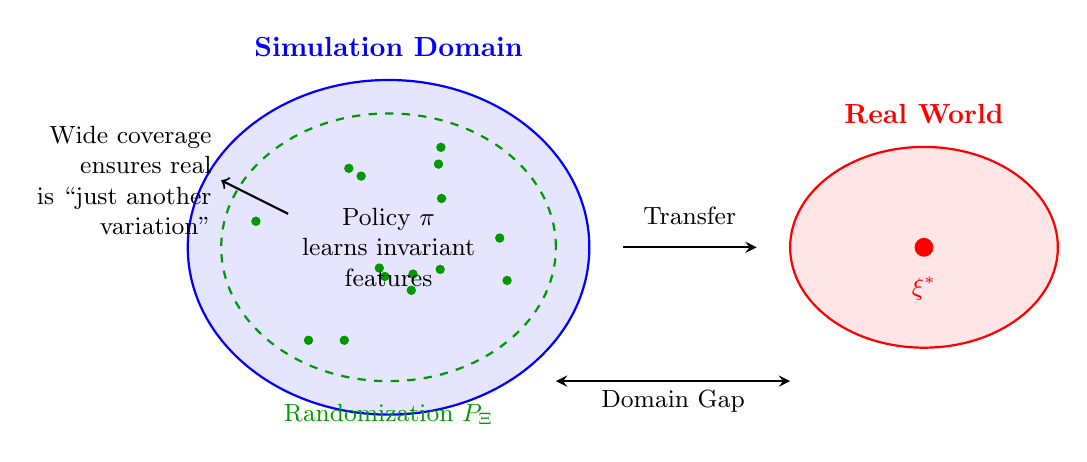
\begin{tikzpicture}[scale=0.85]
    % Simulation domain (large ellipse on left)
    \draw[thick, blue, fill=blue!10] (-4, 0) ellipse (3cm and 2.5cm);
    \node[blue, font=\bfseries] at (-4, 3) {Simulation Domain};

    % Real world domain (smaller ellipse on right)
    \draw[thick, red, fill=red!10] (4, 0) ellipse (2cm and 1.5cm);
    \node[red, font=\bfseries] at (4, 2) {Real World};

    % Randomization distribution (contained in simulation)
    \draw[thick, green!60!black, dashed] (-4, 0) ellipse (2.5cm and 2cm);
    \node[green!60!black, font=\small] at (-4, -2.5) {Randomization $P_\Xi$};

    % Sample points in randomization distribution
    \foreach \i in {1,...,15} {
        \pgfmathsetmacro{\rx}{-4 + 2*rand}
        \pgfmathsetmacro{\ry}{1.5*rand}
        \fill[green!60!black] (\rx, \ry) circle (2pt);
    }

    % Real world point
    \fill[red] (4, 0) circle (4pt);
    \node[red, font=\small, below] at (4, -0.3) {$\xi^*$};

    % Arrow showing transfer
    \draw[thick, ->, >=stealth] (-0.5, 0) -- (1.5, 0);
    \node[above, font=\small] at (0.5, 0.2) {Transfer};

    % Policy learned on randomized data
    \node[font=\small, align=center] at (-4, 0) {Policy $\pi$\\learns invariant\\features};

    % Annotations
    \draw[thick, <->, >=stealth] (-1.5, -2) -- (2, -2);
    \node[below, font=\small] at (0.25, -2) {Domain Gap};

    % Coverage annotation
    \draw[thick, <-] (-6.5, 1) -- (-5.5, 0.5);
    \node[left, font=\small, align=right] at (-6.5, 1) {Wide coverage\\ensures real\\is ``just another\\variation''};

\end{tikzpicture}
\caption{Conceptual illustration of domain randomization. The policy is trained on synthetic data sampled from a distribution $P_\Xi$ over domain parameters (green region). If the distribution provides sufficient coverage and the real-world parameters $\xi^*$ fall within or near this distribution, the policy transfers successfully. The domain gap between simulation and reality is bridged by training on diverse variations.}
\label{fig:domain_randomization}
\end{figure}

\subsection{The Role of Memory in Sim-to-Real Transfer}
\label{subsec:memory_sim2real}

The theoretical analysis of domain randomization reveals a fundamental role for memory in achieving successful sim-to-real transfer. When domain parameters are not directly observable, history-dependent policies can substantially outperform memoryless policies by implicitly inferring domain characteristics from past observations.

Consider a setting where the friction coefficient is unknown but affects the dynamics of object manipulation. A memoryless policy must use a single action for all friction values, leading to suboptimal behavior. A recurrent policy can observe the effects of its actions and infer the friction coefficient, then adapt its strategy accordingly.

\begin{theorem}[Advantage of Memory in Domain Randomization]
\label{thm:memory_advantage}
For domain-randomized MDPs with unobservable domain parameters, let $V^*_{mem}$ denote the optimal value achievable by history-dependent policies and $V^*_{memless}$ denote the optimal value for memoryless policies. Then:
\begin{equation}
V^*_{mem} - V^*_{memless} \geq 0
\end{equation}
with strict inequality when the optimal action depends on unobservable domain parameters.
\end{theorem}

This result has practical implications for architecture design. When using domain randomization for sim-to-real transfer, recurrent neural networks (LSTMs, GRUs) or attention-based architectures that can process sequences of observations may achieve better transfer than feedforward networks. The policy can learn to extract domain-relevant information from the observation history and condition its behavior on this implicit domain estimate.

For object detection specifically, while individual frame processing is typical, incorporating temporal context through video-based detection or tracking-by-detection approaches may improve robustness to domain shift by allowing the model to adapt to the statistics of the target domain during inference.

\section{Multi-Fidelity Optimization}
\label{sec:multi_fidelity}

Multi-fidelity optimization methods exploit the availability of cheaper, lower-fidelity approximations to the expensive target objective. In the context of synthetic data optimization, lower fidelity might correspond to training with fewer images, fewer epochs, smaller model sizes, or reduced image resolution. These methods can dramatically reduce the total computational cost of optimization.

\subsection{Successive Halving Algorithm}
\label{subsec:successive_halving}

Successive Halving provides a principled approach to allocating resources among a set of configurations by iteratively eliminating the worst performers.

\begin{definition}[Successive Halving]
\label{def:successive_halving}
Given $n$ configurations and a total budget $B$, Successive Halving proceeds as follows:
\begin{enumerate}
\item Initialize: $S_0 = \{$all $n$ configurations$\}$, budget per configuration $r_0 = B/(n \lceil \log_\eta n \rceil)$
\item For round $k = 0, 1, \ldots, \lceil \log_\eta n \rceil - 1$:
    \begin{enumerate}
    \item Evaluate each configuration in $S_k$ with budget $r_k$
    \item Keep top $1/\eta$ fraction: $S_{k+1} = \text{top}_{|S_k|/\eta}(S_k)$
    \item Increase budget: $r_{k+1} = r_k \cdot \eta$
    \end{enumerate}
\item Return the best configuration from $S_{\lceil \log_\eta n \rceil}$
\end{enumerate}
where $\eta > 1$ is the reduction factor (typically $\eta = 3$).
\end{definition}

\begin{algorithm}[htbp]
\caption{Successive Halving}
\label{alg:successive_halving}
\begin{algorithmic}[1]
\Require Set of configurations $\mathcal{C}$, total budget $B$, reduction factor $\eta$
\State $n \leftarrow |\mathcal{C}|$, $s_{\max} \leftarrow \lfloor \log_\eta n \rfloor$
\State $r \leftarrow B / (n \cdot (s_{\max} + 1))$ \Comment{Initial budget per configuration}
\State $S \leftarrow \mathcal{C}$ \Comment{Active configurations}
\For{$k = 0, 1, \ldots, s_{\max}$}
    \State $n_k \leftarrow \lfloor n / \eta^k \rfloor$ \Comment{Number of configurations in round $k$}
    \State $r_k \leftarrow r \cdot \eta^k$ \Comment{Budget per configuration in round $k$}
    \State $L \leftarrow \{(\text{config}, \text{Evaluate}(\text{config}, r_k)) : \text{config} \in S\}$
    \State $S \leftarrow \text{top}_{n_k / \eta}(L)$ \Comment{Keep best $n_k/\eta$ configurations}
\EndFor
\State \Return Configuration in $S$ with best final evaluation
\end{algorithmic}
\end{algorithm}

The key assumption underlying Successive Halving is that the ranking of configurations is approximately preserved across fidelity levels: configurations that perform well with small budgets tend to perform well with larger budgets. When this assumption holds, Successive Halving can identify the best configuration with far less total computation than exhaustive evaluation.

\begin{figure}[htbp]
\centering
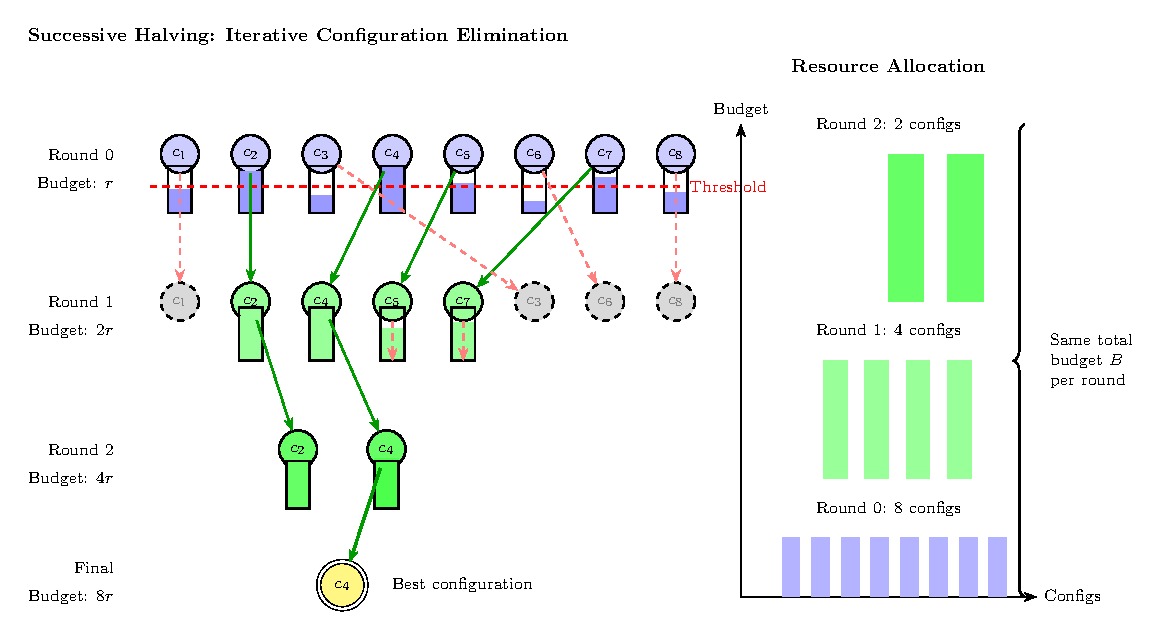
\includegraphics[width=0.95\textwidth]{figures/ch02_fig4_successive_halving.pdf}
\caption{Successive Halving for multi-fidelity hyperparameter optimization. Left: The algorithm iteratively evaluates configurations with increasing budgets while eliminating the bottom half at each round. Starting with 8 configurations (Round 0), only 4 survive to Round 1, then 2 to Round 2, with the final round identifying the best configuration. Right: Resource allocation across rounds shows how the same total budget is distributed---initially spread across many configurations with small budgets, then concentrated on fewer promising configurations with larger budgets. This approach efficiently explores the configuration space while avoiding wasted computation on poor performers.}
\label{fig:successive_halving}
\end{figure}

\subsection{Hyperband Framework}
\label{subsec:hyperband}

Hyperband addresses a fundamental limitation of Successive Halving: the algorithm requires specifying the number of configurations $n$ in advance, which implicitly determines the trade-off between exploration (many configurations, small initial budgets) and exploitation (few configurations, large initial budgets).

\begin{definition}[Hyperband]
\label{def:hyperband}
Hyperband runs multiple instances of Successive Halving with different exploration-exploitation trade-offs:
\begin{equation}
s \in \{s_{\max}, s_{\max}-1, \ldots, 0\}
\end{equation}
where $s_{\max} = \lfloor \log_\eta(R) \rfloor$ and $R$ is the maximum budget per configuration. For each $s$, Successive Halving is run with:
\begin{align}
n_s &= \left\lceil \frac{(s_{\max} + 1) \cdot \eta^s}{s + 1} \right\rceil \text{ configurations} \\
r_s &= R \cdot \eta^{-s} \text{ initial budget}
\end{align}
\end{definition}

\begin{algorithm}[htbp]
\caption{Hyperband}
\label{alg:hyperband}
\begin{algorithmic}[1]
\Require Maximum budget per configuration $R$, reduction factor $\eta$
\Require Configuration sampling function GetConfiguration()
\State $s_{\max} \leftarrow \lfloor \log_\eta R \rfloor$, $B \leftarrow (s_{\max} + 1) R$
\For{$s \in \{s_{\max}, s_{\max}-1, \ldots, 0\}$} \Comment{Outer loop over brackets}
    \State $n \leftarrow \lceil B \cdot \eta^s / (R \cdot (s+1)) \rceil$ \Comment{Initial number of configurations}
    \State $r \leftarrow R \cdot \eta^{-s}$ \Comment{Initial budget per configuration}
    \State $T \leftarrow \{\text{GetConfiguration}() : i = 1, \ldots, n\}$ \Comment{Sample configurations}
    \For{$i \in \{0, 1, \ldots, s\}$} \Comment{Inner Successive Halving loop}
        \State $n_i \leftarrow \lfloor n \cdot \eta^{-i} \rfloor$, $r_i \leftarrow r \cdot \eta^i$
        \State $L \leftarrow \{(\text{config}, \text{Evaluate}(\text{config}, r_i)) : \text{config} \in T\}$
        \State $T \leftarrow \text{top}_{n_i / \eta}(L)$
    \EndFor
\EndFor
\State \Return Best configuration observed across all brackets
\end{algorithmic}
\end{algorithm}

Hyperband's outer loop (varying $s$) explores different trade-offs: large $s$ corresponds to aggressive early stopping with many configurations, while small $s$ provides more resources per configuration. This hedge ensures robust performance regardless of how well early performance predicts final performance.

\subsection{BOHB: Combining Bayesian Optimization with Hyperband}
\label{subsec:bohb}

BOHB (Bayesian Optimization HyperBand) combines the sample efficiency of Bayesian optimization for guiding configuration sampling with the early stopping benefits of Hyperband.

\begin{definition}[BOHB]
\label{def:bohb}
BOHB replaces the random sampling in Hyperband with model-based sampling using a Tree-structured Parzen Estimator (TPE) or kernel density estimator:
\begin{enumerate}
\item Maintain a surrogate model fitted to all observations at each fidelity level
\item Sample configurations by optimizing an acquisition function over the surrogate model
\item Use Hyperband's scheduling to allocate resources across configurations
\item Transfer knowledge across fidelity levels using a weighted combination of models
\end{enumerate}
\end{definition}

The TPE model in BOHB separately models the density of good configurations $\ell(x) = p(x | y < y^*)$ and the density of other configurations $g(x) = p(x | y \geq y^*)$. New configurations are sampled by maximizing the ratio $\ell(x)/g(x)$, which approximates expected improvement.

BOHB maintains separate density models for each fidelity level but uses a weighted combination based on the number of observations at each level. This allows knowledge transfer from cheaper low-fidelity evaluations to guide high-fidelity search.

\begin{table}[htbp]
\centering
\caption{Comparison of Multi-Fidelity Optimization Methods}
\label{tab:multi_fidelity}
\begin{tabular}{lccc}
\toprule
\textbf{Method} & \textbf{Configuration Selection} & \textbf{Early Stopping} & \textbf{Parallelization} \\
\midrule
Random Search & Uniform random & No & Embarrassingly parallel \\
Successive Halving & Uniform random & Yes (aggressive) & Within brackets \\
Hyperband & Uniform random & Yes (hedged) & Across brackets \\
BOHB & Model-based (TPE) & Yes (hedged) & Across brackets \\
\bottomrule
\end{tabular}
\end{table}

For the problem of synthetic data optimization, multi-fidelity methods offer substantial computational savings. The fidelity dimension can correspond to the number of synthetic training images, the number of training epochs, or the complexity of the detection model. Early termination of unpromising configurations prevents wasting computational resources on parameter settings that yield poor detection performance.

\section{Summary}
\label{sec:background_summary}

This chapter has established the theoretical foundations necessary for developing reinforcement learning approaches to synthetic dataset optimization for object detection. We examined the evolution of object detection architectures, with particular emphasis on the YOLO family that provides the target application for our optimization framework. The mathematical foundations of reinforcement learning were developed, including Markov Decision Processes, policy gradient methods (TRPO, PPO), and actor-critic architectures (SAC, TD3). Bayesian optimization was presented as a complementary approach with strong sample efficiency properties. Domain randomization theory was formalized, establishing conditions under which training on randomized synthetic data enables successful transfer to real-world domains. Finally, multi-fidelity optimization methods including Successive Halving, Hyperband, and BOHB were introduced as techniques for efficiently exploring expensive objective functions.

The subsequent chapters build on these foundations to develop our framework for using reinforcement learning to optimize synthetic data generation parameters. Chapter 3 formalizes the problem as an MDP and defines the state space, action space, and reward function. Chapter 4 presents our algorithmic approach combining elements of the methods introduced here. Chapter 5 provides experimental validation on real-world object detection benchmarks.
